\documentclass{article}

\usepackage{graphicx}
\usepackage{tikz}
\usepackage{tikzsymbols}
\usetikzlibrary{calc,patterns,shapes.geometric}
\pagestyle{empty}
\usepackage[margin=0pt]{geometry}
\geometry{papersize={14in,12in}}

\def\centerarc[#1](#2)(#3:#4:#5){\draw[#1] ($(#2)+({#5*cos(#3)},{#5*sin(#3)})$) arc (#3:#4:#5);}

\begin{document}
	\begin{figure}
		\centering
		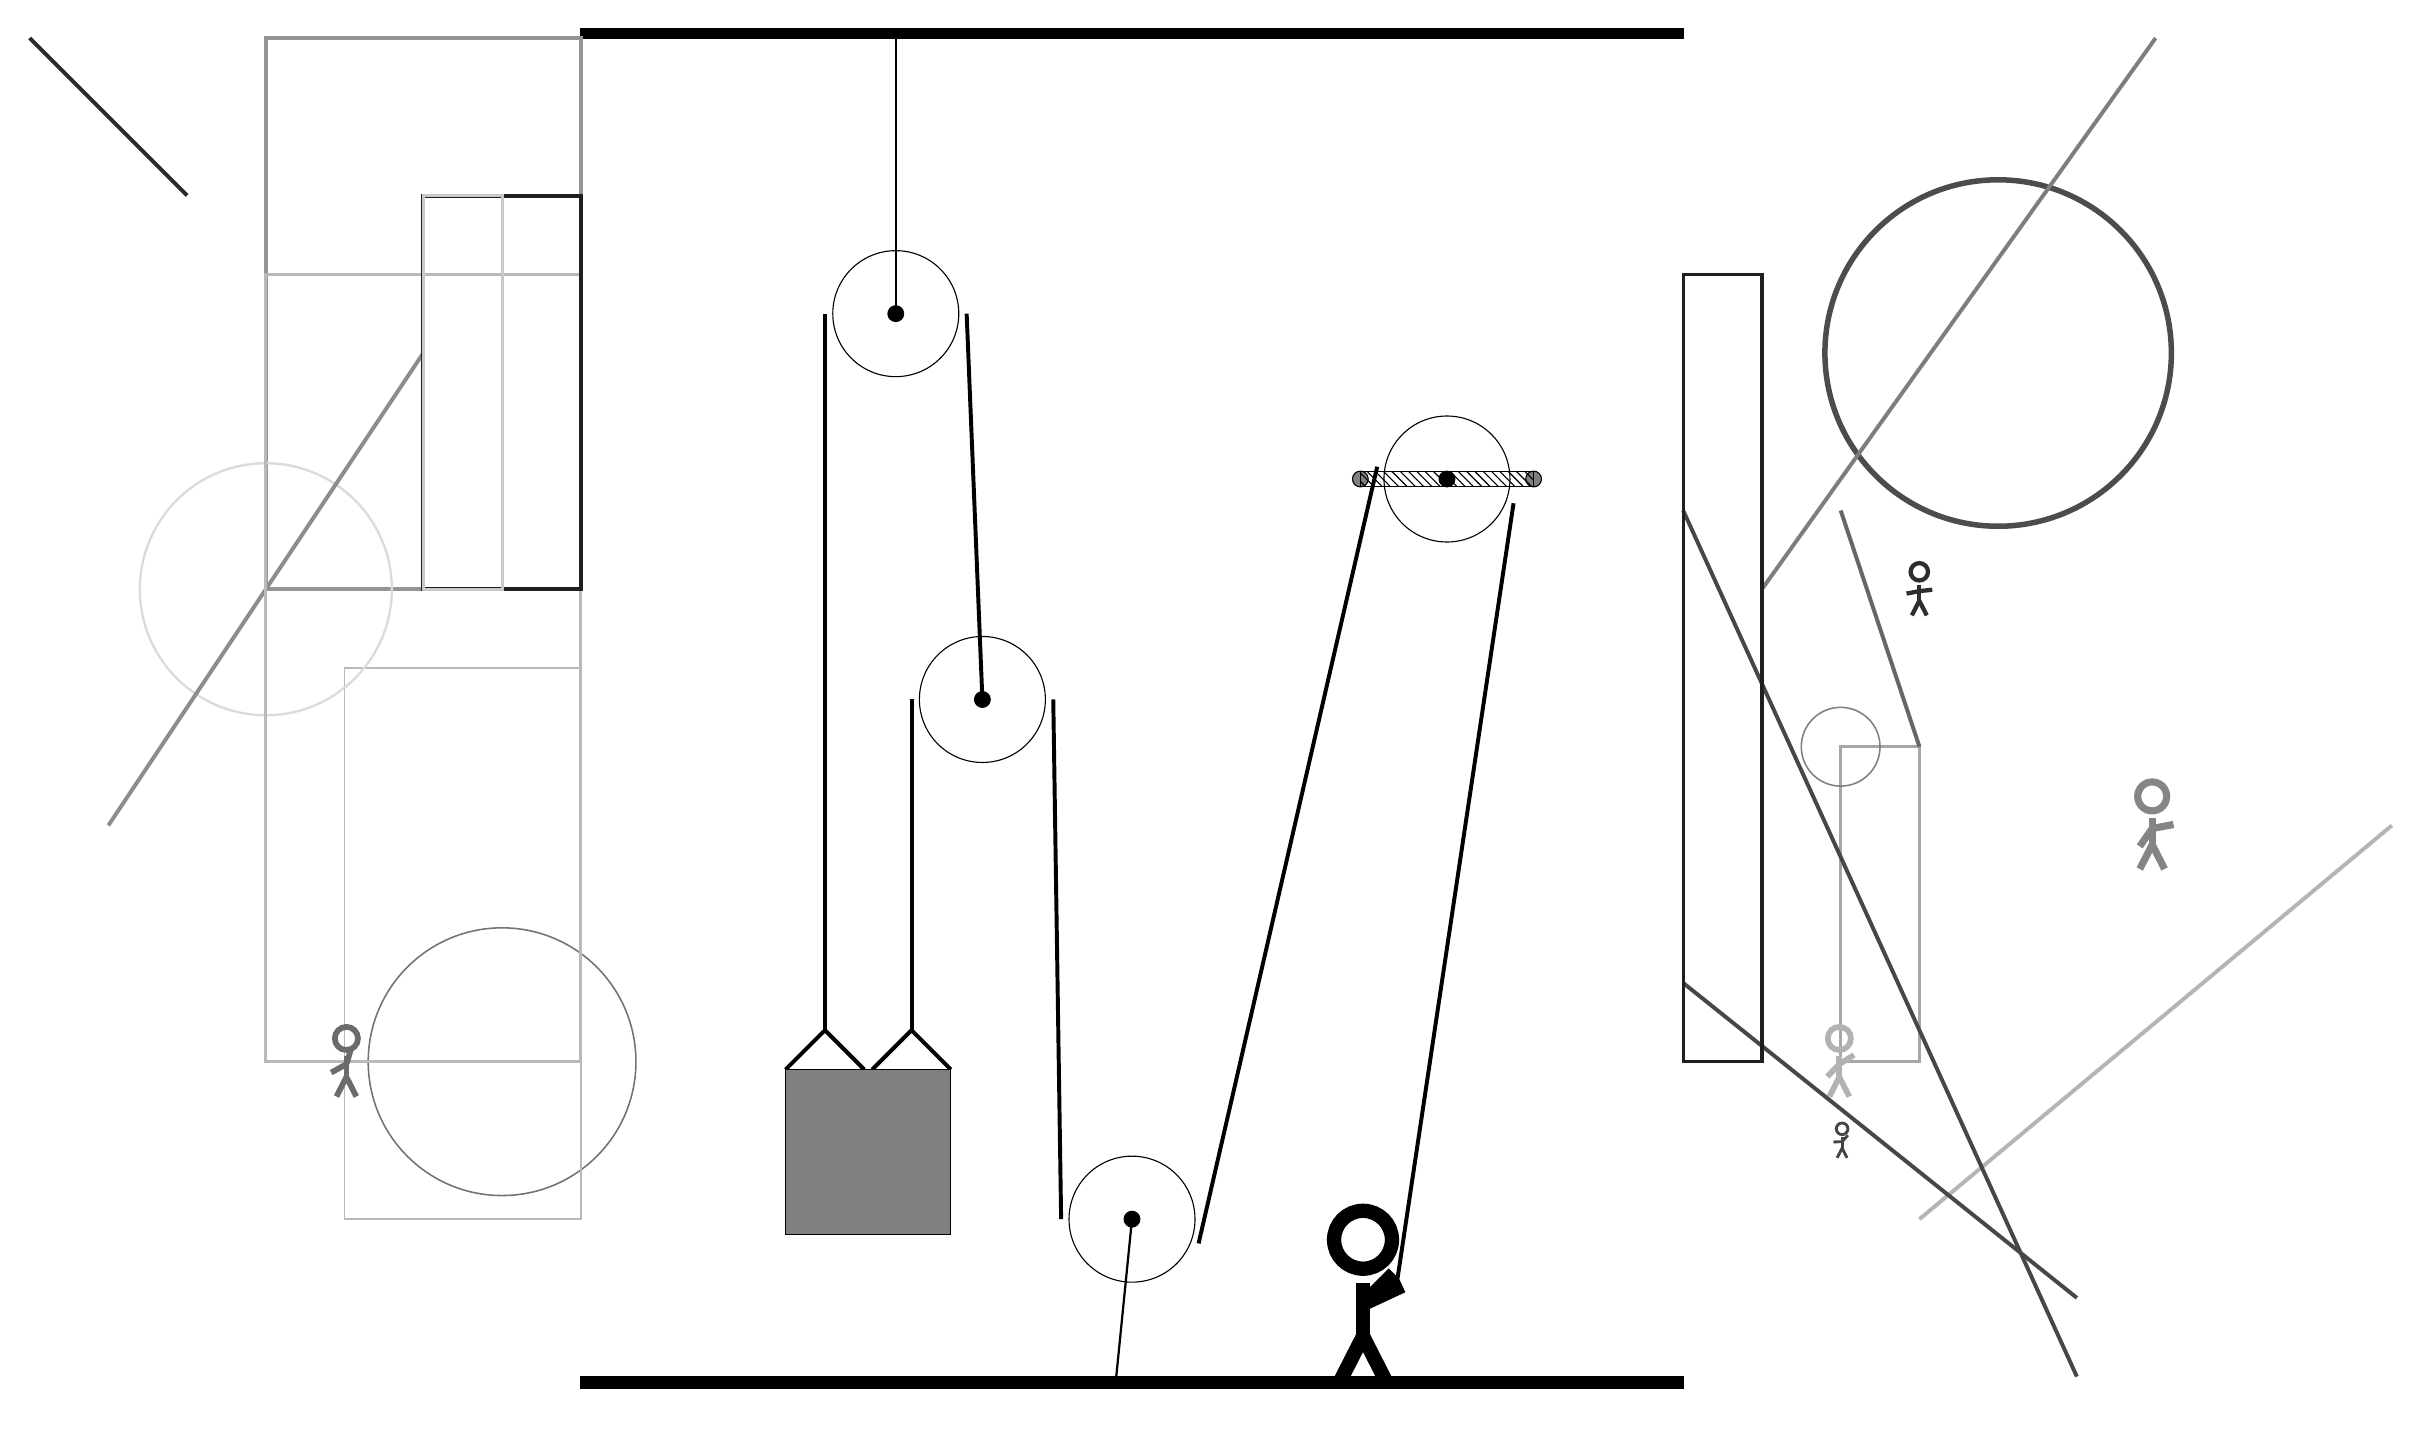
\begin{tikzpicture}
			%%%%% START %%%%%
			
			\draw[fill=black] (-2, 14) rectangle (12, 14.125);
			
			\draw (2, 10.5) circle (0.8);
			\draw[fill=black] (2, 10.5) circle (0.1);
			\draw[thick] (2, 10.5) -- (2, 14);
			
			\draw (3.1, 5.6) circle (0.8);
			\draw[fill=black] (3.1, 5.6) circle (0.1);
			
			\draw (5, -1) circle (0.8);
			\draw[fill=black] (5, -1) circle (0.1);
			\draw[thick] (5, -1) -- (4.8, -3);
			
			\draw (9, 8.4) circle (0.8);
			\draw[fill=black] (9, 8.4) circle (0.1);
			\draw[fill=black!50] (7.9, 8.4) circle (0.1);
			\draw[fill=black!50] (10.1, 8.4) circle (0.1);
			\draw[pattern=north west lines, pattern color=black] (7.9, 8.5) rectangle (10.1, 8.3);
			
			\draw[line width = 0.5mm]  (0.6, 0.9) -- (1.1, 1.4) -- (1.6, 0.9);
			\draw[line width = 0.5mm]  (1.7, 0.9) -- (2.2, 1.4) -- (2.7, 0.9);
			\draw[fill=black!50] (0.6, 0.9) rectangle (2.7, -1.2);
			
			\node[line width=0.5mm, color=black!48] at (18, 4) {\Strichmaxerl[5][55][11]};
			
			\draw [line width=0.2mm, color=black!55](-3, 1) circle (1.7);
			\draw[line width=0.5mm, color=black!29](15, -1) -- (21, 4);
			\draw[line width=0.4mm, color=black!35] (14, 1) rectangle (15, 5);
			\draw[line width=0.5mm, color=black!42] (-2, 7) rectangle (-6, 14);
			
			\draw [line width=0.2mm, color=black!50](14, 5) circle (0.5);
			\node[line width=0.3mm, color=black!30] at (14, 1) {\Strichmaxerl[4][46][32]};
			\draw [line width=0.7mm, color=black!70](16, 10) circle (2.2);
			\draw[line width=0.2mm, color=black!28] (-2, -1) rectangle (-5, 6);
			\draw[line width=0.5mm, color=black!83](-7, 12) -- (-9, 14);
			
			\draw[line width=0.5mm, color=black!72](17, -2) -- (12, 2);
			
			\draw[line width=0.5mm, color=black!51](13, 7) -- (18, 14);
			\node[line width=0.6mm, color=black!82] at (15, 7) {\Strichmaxerl[3][11][6]};
			
			\draw [line width=0.3mm, color=black!14](-6, 7) circle (1.6);
			\node[line width=0.5mm, color=black!73] at (14, 0) {\Strichmaxerl[2][2][48]};
			\draw[line width=0.5mm, color=black!60](14, 8) -- (15, 5);
			
			\draw[line width=0.5mm, color=black!45](-4, 10) -- (-8, 4);
			\draw[line width=0.4mm, color=black!27] (-2, 1) rectangle (-6, 11);
			\draw[line width=0.5mm, color=black!72](17, -3) -- (12, 8);
			\draw[line width=0.4mm, color=black!88] (13, 1) rectangle (12, 11);
			\draw[line width=0.5mm, color=black!88] (-4, 12) rectangle (-2, 7);
			
			\node[line width=0.4mm, color=black!58] at (-5, 1) {\Strichmaxerl[4][29][73]};
			
			\draw[line width=0.4mm, color=black!21] (-3, 12) rectangle (-4, 7);
			
			\draw[line width = 0.5mm] (1.1, 10.5) -- (1.1, 1.4);
			\centerarc[line width = 0.5mm](2, 10.5)(0:180:0.9);
			\draw[line width = 0.5mm] (2.9, 10.5) -- (3.1, 5.6);
			\draw[line width = 0.5mm] (2.2, 5.6) -- (2.2, 1.4);
			\centerarc[line width = 0.5mm](3.1, 5.6)(0:180:0.9);
			\draw[line width = 0.5mm] (4.0, 5.6) -- (4.1, -1);
			\centerarc[line width = 0.5mm](5, -1)(180:340:0.9);
			\draw[line width=0.5mm](5.8457, -1.3078) -- (8.1137, 8.5562);
			\centerarc[line width = 0.5mm](9, 8.4)(-20:170:0.9);
			\draw[line width=0.5mm](9.8457, 8.0922) --  (8.35, -1.9);
			
			\node at (8, -2) {\Strichmaxerl[10][225][25]};
			
			\draw[fill=black] (-2, -3) rectangle (12, -3.15);
			
			%%%%% END %%%%%
		\end{tikzpicture}
	\end{figure}	
\end{document}